\documentclass[aspectratio=169]{beamer}
\usetheme{Madrid}
\usecolortheme{beaver}
\usepackage[utf8]{inputenc}
\usepackage[T1]{fontenc}
\usepackage{tikz}
\usepackage{amssymb}
\usepackage{graphicx}
\setbeamertemplate{navigation symbols}{}
\setbeamercolor{title}{fg=white,bg=cyan!60!black}
\setbeamercolor{frametitle}{fg=white,bg=cyan!50!black}
\setbeamercolor{block title}{bg=cyan!15,fg=black}
\setbeamercolor{block body}{bg=cyan!5,fg=black}

\title{G3 — Decisions}
\subtitle{Lesson 1: Traffic Light}
\author{ByteForge --- Grade 7 --- Game Maker}
\date{}

\begin{document}

\begin{frame}
    \titlepage
\end{frame}

\begin{frame}{IF/ELSE — choosing between paths}
    \Large
    An IF only runs when a condition is true. Chaining IF/ELSE IF/ELSE picks between three outcomes — only one branch ever runs.

    \begin{center}
    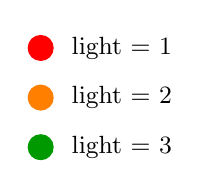
\begin{tikzpicture}[scale=0.9]

        \filldraw[red] (0,0) circle (5pt);
        \filldraw[orange] (0,-0.7) circle (5pt);
        \filldraw[green!60!black] (0,-1.4) circle (5pt);
        \node[right] at (0.3,0) {\small light = 1};
        \node[right] at (0.3,-0.7) {\small light = 2};
        \node[right] at (0.3,-1.4) {\small light = 3};
    \end{tikzpicture}
    \end{center}
\end{frame}

\begin{frame}{Your Turn}
    \Large
    Open the student map, find \textbf{G3 — Decisions}, and complete
    the \textbf{Traffic Light} challenge --- everything you just saw, they now do themselves.
\end{frame}

\end{document}
